\header{
    \section{Adishatz} \label{adishatz}
    %
    \insertComment{}{}
}

\enluminure{2}{\href{https://lyricstranslate.com/fr/adishatz-au-revoir.html}{L}}{o purmèr} dia d’escola, desvelhat tot doçament,
\\Esbarrit en aqueth mond, hart de plors e de turments,
\\E d'aprèp quauques anadas, cada setmana en pension,
\\Viver drin mei luènh de casa, descobrir d’autas faiçons.
\\\\\textbf{Refrain :}
\\Adishatz, qu’ei a partir!
\\Tornarai, hu bèth matin, amic!
\\Qu’ei aicí qui cal finir,
\\Shens nat brut, shens nat chepic.
\\\\Vint ans, lo bèth atge, sentiment de libertat,
\\Qu’èra lo temps de la hèsta, de cantar nòsta amistat.
\\Las purmèras amoretas debat lo ceu estelat,
\\En los uèlhs d’ua gojata a qui no calguèt pas deishar...
\\\\Cal ganhar la sua vita, qu’ei sovent luènh deu país,
\\Lo trabalh deus joens d'ara, que'us a miat dinc a París.
\\Alavetz tà las vacanças, que vienen passar l’estiu
\\Au còr d’un petit vilatge, arrosat per noste arriu.
\\\\\textbf{Traduction : }
\\Le premier jour d'école, doucement réveillé,
\\Égaré dans ce monde, rempli de pleurs et de tourment,
\\Et après quelques années, chaque semaine en pension,
\\Vivre plus loin de chez soi, découvrir d'autres façons.
\\\\Au revoir, c'est parti !
\\Je reviendrai par un beau matin, l'ami !
\\C'est ici qu'il nous faut finir,
\\Sans querelle ni tracas.
\\\\Vingt ans, déjà le bel âge, un sentiment de liberté
\\Ce fut un temps de fête, en chantant notre amitié.
\\Les premiers amours, couverts d'un ciel étoilé
\\Dans les yeux d'une jeune fille qu'il ne fallait pas quitter.
\breakpage
\\\\Gagner souvent nécessite souvent de quitter le pays,
\\Aujourd'hui le travail des jeunes les envoie jusqu'à Paris.
\\Et donc pendant les vacances, ils viennent passer l'été
\\Au cœur d'un petit village arrosé de notre ruisseau.

\vspace{1cm}
\begin{center}
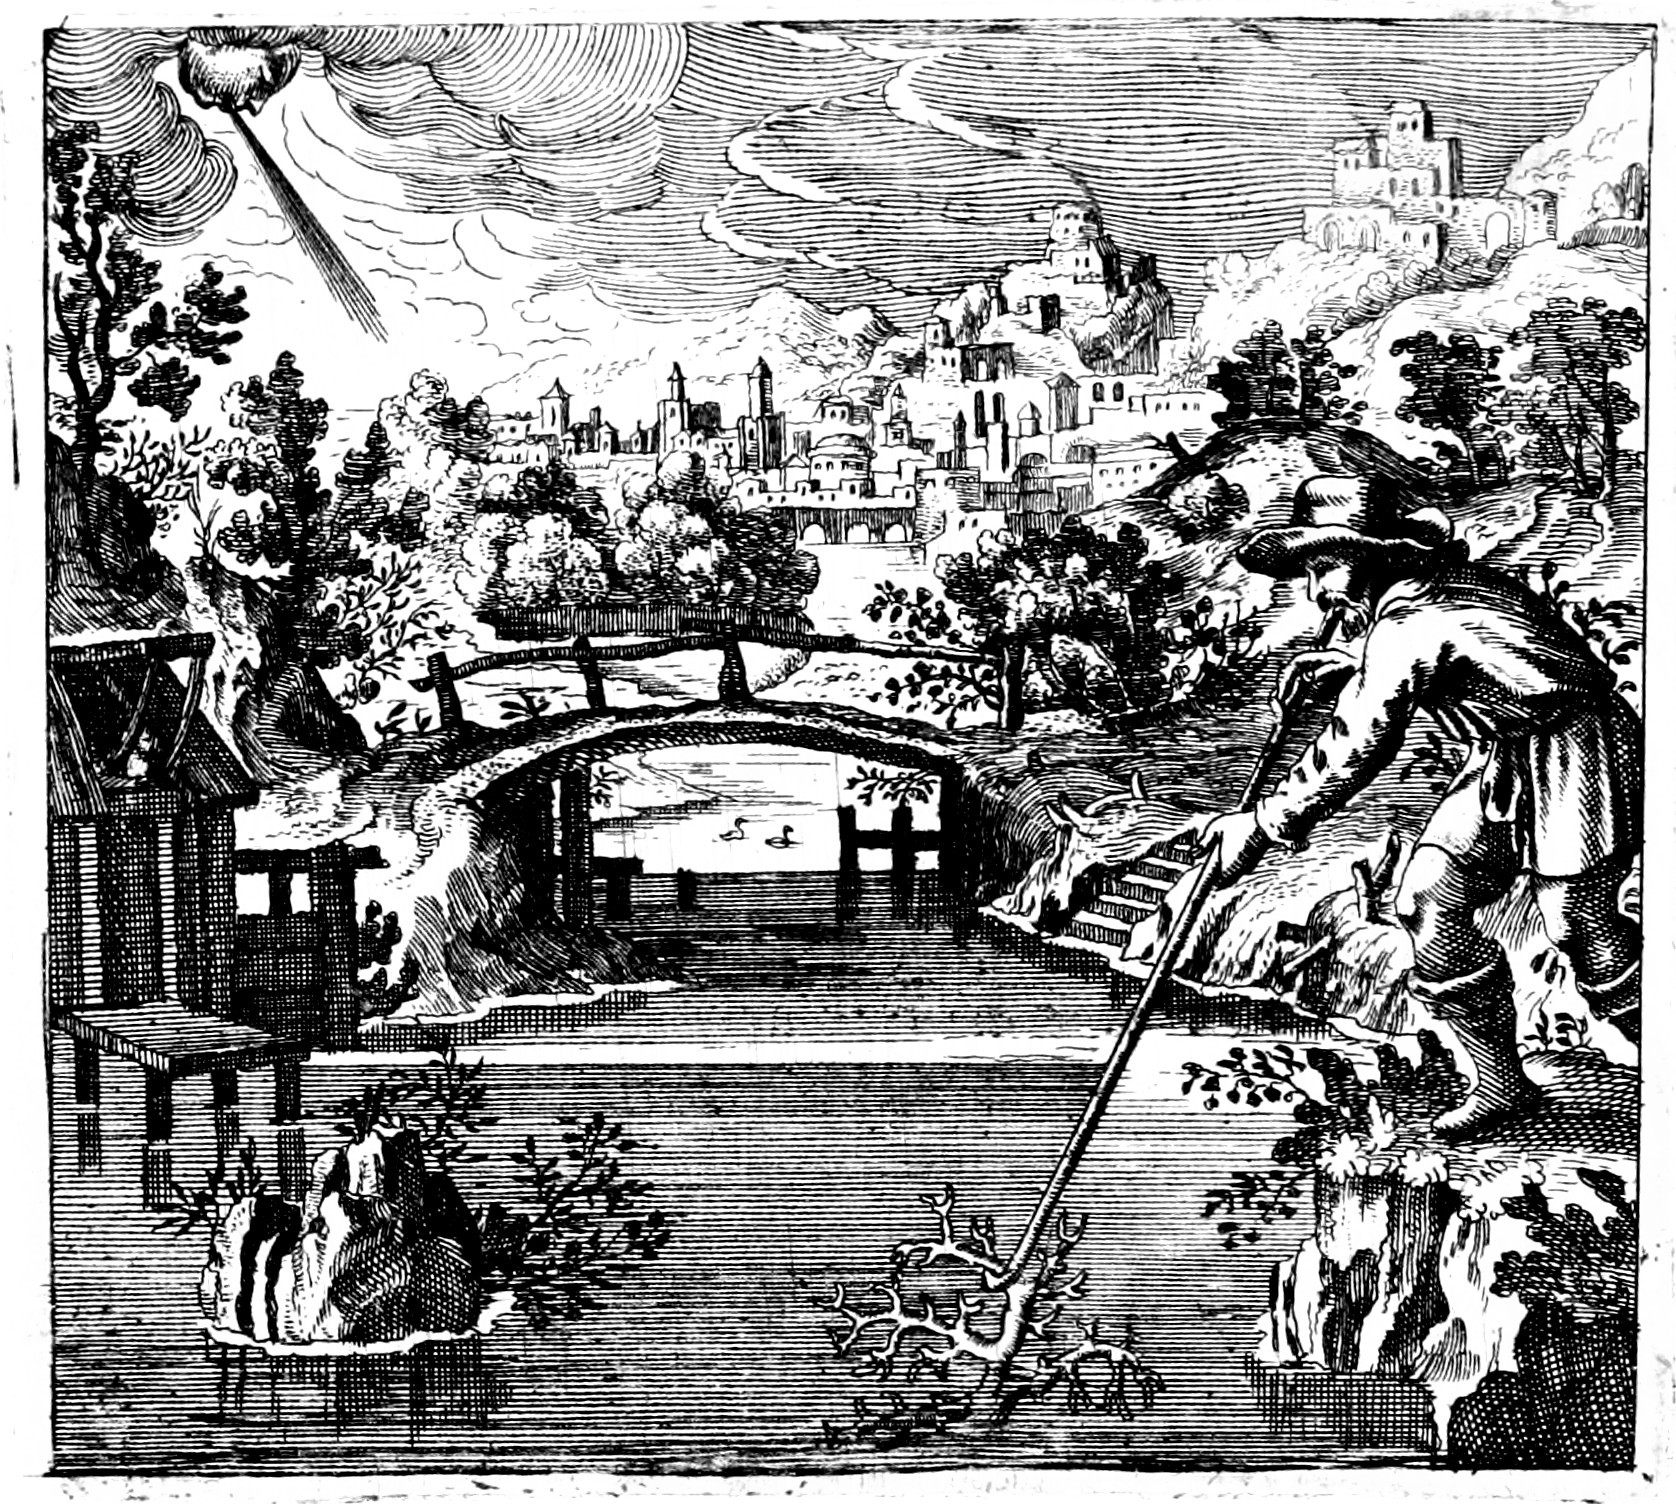
\includegraphics[width=1\textwidth]{images/brev33.png}
\end{center}

\breakpage